\documentclass[letter]{article}

\usepackage[english]{babel}
\usepackage[utf8]{inputenc}
\usepackage{amsmath}
\usepackage[colorinlistoftodos]{todonotes}
\usepackage{makecell}
\usepackage{multirow}
\usepackage{caption}
\usepackage{subcaption}
\usepackage{graphicx}
\usepackage{hyperref}
\usepackage{float}
\usepackage[all]{hypcap}
\usepackage[space]{grffile}
\usepackage{enumitem}

\newlist{questions}{enumerate}{1}
\setlist[questions, 1]{label = \arabic*}
\newlist{bonus}{enumerate}{1}
\setlist[bonus, 1]{label = Bonus \arabic*}



% Adjust margins
\addtolength{\oddsidemargin}{-0.75in}
\addtolength{\evensidemargin}{-0.75in}
\addtolength{\textwidth}{1.5in}
\addtolength{\topmargin}{-.5in}
\addtolength{\textheight}{1.5in}

\title{CS 520: Assignment 2 - MineSweeper, Inference-Informed Action}
\author{Haoyang Zhang, Han Wu, Shengjie Li, Zhichao Xu}
\date{\today}

\begin{document}
\maketitle

\section{Introduction, group members and division of workload}
\label{sec:Introduction}

In this group project, apart from implementing DFS, BFS, $ A^* $ with Euclidean Distance Heuristic and $ A^* $ with Manhattan Distance Heuristic, we also did some modification to these algorithms for different performance out of our personal interests.  \\
\begin{tabular}{| p{2.5cm} | p{\textwidth -3.5cm} |}
	\hline
	\makecell[c]{Name \\ RUID} & Workload \\
	\hline
	\makecell[c]{Haoyang Zhang \\ 188008687} & {Implemented DFS, Iterative Deepening DFS, BFS, Bidirectional BFS, Bidirectional $ A^* $, Simulated-Annealing-Based Beam Search and the visualization of maze. Modified DFS to make it able to return optimal path. Added Last-in First-out feature to $ A^* $. Managed to combine Simulated-Annealing-Based Beam Search with Genetic Algorithm. Ran tests for DFS and BFS in question 10. Finished half of the writing of report for part 2.} \\
	\hline
	\makecell[c]{Han Wu \\ 189008460} & {Wrote python scripts for testing the performance of algorithms. Combine the data and generated figures for question 1, 2, 4 and 5. Finished the writing of report for question 1, 2, 4 and 5.} \\
	\hline
	\makecell[c]{Shengjie Li \\ 188008047} & {Implemented $ A^* $ with Euclidean Distance Heuristic, $ A^* $ with Manhattan Distance Heuristic and Genetic Algorithm. Ran tests for $ A^* $ with Euclidean Distance Heuristic and Manhattan Distance inquestion 10. Finished the format design of whole report using \LaTeX. } \\
	\hline
	\makecell[c]{Zhichao Xu \\ 188008912} & {Wrote python scripts for testing the performance of algorithms. Combine the data and generated figures for question 3, 6 and 7. Finished the writing of report for question 3, 6 and 7. Suggested an improvement of $ A^* $ using Chebyshev Distance.} \\
	\hline
\end{tabular}


\section{Questions and Writeup}
\label{sec:Questions and Writeup}
\begin{enumerate}
	\item {Representation: How did you represent the board in your program, and how did you represent the information / knowledge that clue cells reveal?} \\
	\\
	In our program, the basic board is represented by a matrix, which is constructed by a 2-dimensional array. For example, a $ 64 \times 64 $ board is represented by an array of 64 elements, and each element is an array with length of 64. 
	
	The board is represented by 4 matrices:  “covered”, “flag”,  “\_mine” and “\_clue”. The matrix “covered” saves exploration status. 
	\begin{itemize}
		\item {The matrix “flag” records blocks that agents regard as mines.} 
		\item {The matrix “\_mine” represents the distribution of mines.} 
		\item {The matrix “\_clue” is a preprocessed matrix that records each block’s hint number.} 
		\item {The hint number here is used to save time when solving minesweeper.} 
	\end{itemize}   
	
	The knowledge base is represented by 9 matrices: “covered”, “safe”, “flag”, “hint”, “warn”, “left”, “done”, “nebr” and “prob”. 
	\begin{itemize}
		\item {Matrix “covered” and “flag” are the same as the board’s matrix.}
		\item {Matrix “safe” records the blocks that agents regard as safe blocks.}
		\item {Matrix “hint” saves the hint number the agents have got from the minesweeper.}
		\item {Matrix “warn” represents the number of each hint block’s un-flagged mines. \\ Namely, $ \text{warn} = \text{hint} - (\text{the number of neighbor flags}) $.}
		\item {Matrix “left” represents the number of each block’s inconclusive neighbors. \\ Namely, $ \text{left} = 8 - \text{(the number of neighbor flags-the number of neighbor uncovered)} - \text{(edge cost)} $.}
		\item {Matrix “done” records blocks whose neighbors are all conclusive. Such blocks could be ignored when agents are solving the minesweeper.}
		\item {Matrix “nebr” is a hash value matrix. It records the inconclusive neighbors of each block. Agents use it when trying to solve equations like “$ A+B+C=2 $, $ A+B=1 $”.}
		\item {Matrix “prob” is actually a tensor. It records each block’s probability of being a mine block, given each neighbor’s data. Therefore, the size of “prob” is $ rows \times columns \times 9 $ (with an extra basic probability).}
	\end{itemize}         
	
	\item {Inference: When you collect a new clue, how do you model / process / compute the information you gain from it? i.e., how do you update your current state of knowledge based on that clue? Does your program deduce everything it can from a given clue before continuing? If so, how can you be sure of this, and if not, how could you consider improving it?} \\
	\\
	There are at least 3 things we need to do:
	\begin{enumerate}
		\item {Compute “warn” value of the block we have just explored.}
		\item {Update all neighbors’ “left” and “nebr” value.}
		\item {Update all these 9 blocks’ neighbor’s “prob” value.}
	\end{enumerate}
	
	If the updated "prob" value of a block is 0 or 1, it is now conclusive. Therefore, we add this block to the waiting line, to be explored or marked flag in the future.
	
	Sure that there are many other things we might make deductions, for instance, trying to combine it with a clue we have already known. However, there is a reason for stopping combining clues. Combining clues is especially time-consuming without a proper direction or heuristic. For a given knowledge base, the statements we can deduce do not change, even if we add more hints into the knowledge base. Therefore, it is not economical to spend so much time combining clues when we can explore and make deductions from somewhere else, because new hints may easily lead to exactly the same statements.
	
	If we have nothing else to do, there are still several ways to combine them (the detailed introduction is in “$\backslash$docs$\backslash$Solution Algorithm Explanation.html”). The structure of some hints (value relationship and geometric relationship) tends to be solvable, and then we can focus on those structures. At least, we can use proof by contradiction to combine a large number of hints at one time, though it is also time-consuming.
	
	\item {Decisions: Given a current state of the board, and a state of knowledge about the board, how does your program decide which cell to search next? Are there any risks, and how do you face them?} \\
	\\
	There are mainly 4 things we can do:
	\begin{enumerate}
		\item {If there is a block in the waiting line, process it. \\ This brings no risk and is the easiest thing we can do.}
		\item {Use pattern recognition method to find a group of blocks that usually solvable, and try to solve it. \\ This performs surprisingly well, and takes not that much time, comparing with proof by contradiction.}
		\item {Use constraint satisfaction and proof by contradiction to find a conclusive block. \\ Pattern recognition could miss complex solvable structures, and therefore, we use the former one to improve. But generally, it takes too much time. Also, it has limitations. For example, it chooses some blocks randomly to search rather than choose all inconclusive blocks. Note that this limitation also leads to the missing of some solvable blocks.}
		\item {Should all attempts above fail, find a block that is worthy to take the risk to open. \\ The block should be either with the lowest risk, or “well-paid”. A “well-paid” block is a block whose clue is expected to play an important role in the solving process in the future if the block itself is not a mine.}
	\end{enumerate}
	
	\item {Performance: For a reasonably-sized board and a reasonable number of mines, include a play-by-play progres- sion to completion or loss. Are there any points where your program makes a decision that you don’t agree with? Are there any points where your program made a decision that surprised you? Why was your program able to make that decision?} \\
	
	TODO \\
	
	\item {Performance: For a fixed, reasonable size of board, what is the largest number of mines that your program can still usually solve? Where does your program struggle?} \\
	\\
	We used the size of $ 64 \times 64 $ as the board size. From our preliminary testing result, our program can solve board of less than $ 20\% $ mine density easily. When the mine density is over $ 20\% $, it usually takes a much longer time. The threshold for the board to become not solvable for our program is $ 23\% $. When the mine density is over $ 23\% $, nearly all the boards are not solvable for our program. We increased the number of experiments, setting mine density to less than $ 20\% $, the result is showed in Figure \ref{fig:2}.
	
	\begin{figure}
		\centering
		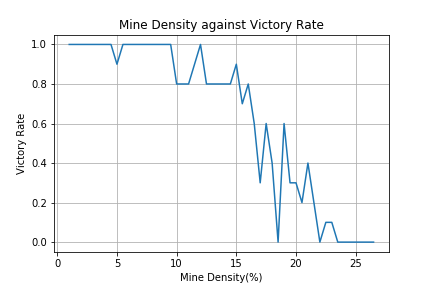
\includegraphics[width=\textwidth]{../pics/Mine-Density-against-Victory-Rate.png}
		\caption{\label{fig:2}Mine Density against Victory Rate.}
	\end{figure}
	
	We have come to the conclusion that our program can confidently solve boards of less than $ 20\% $ mine density. 
	As mine density increases, it takes more time to make a deduction. At the same time, there are more unsolvable scenarios where we have to take risks to explore new blocks. That’s where our program begins to struggle.
	
	\item {Efficiency: What are some of the space or time constraints you run into in implementing this program? Are these problem specific constraints, or implementation specific constraints? In the case of implementation constraints, what could you improve on?} \\
	\item {Improvements: Consider augmenting your program’s knowledge in the following way - when the user inputs the size of the board, they also input the total number of mines on the board. How can this information be modeled and included in your program, and used to inform action? How can you use this information to effectively improve the performance of your program, particularly in terms of the number of mines it can effectively solve.} 
\end{enumerate}


\end{document}